\label{sec:acq}

The KID is a superconducting resonator that measures the density variation of the quasi-particles in the lattice, due to photon absorption. It is read-out by a bias line, injecting a tone at its correspondence resonant frequency; at this peculiar frequency, in fact, the coupling between the resonator and the readout line results in an energy absorption, aka band-stop filter. Its time constant is fixed by the recombination time of the quasi-particles from $10 \mu s$ to $100 \mu s$. This represents a major advantage with respect to competitors that are, indeed, a factor $\gtrsim$10 slower.

The $S_{21}$ signal (output/input ratio) related to the KID detector is studied in the complex plane $(I,Q)$, where the resonance shape corresponds to a circle.
The conversion of the $(I,Q)$ signal to absorbed optical power is one of the most difficult challenge using KIDs and it represents a different issue to readout, e.g., thermal detectors (bolometer, TES et cetera).

\subsection{Circular fitting: necessities and constraints}

Smart readout technique is required to properly study the signal and do not encounter huge amount of data. In the past, e.g. for NIKA, an innovative readout technique has been developed (see \cite{Calvo2013} for a detailed discussion). 
The idea, as described in \cite{Catalano2014} , has been to replace the standard fixed excitation (single frequency) tone with a modulated input based on two different frequencies separated by $f_{LO}$: $f_+ = f_0 + \delta f_{LO}/2$ and o$f_- = f_0 - \delta f_{LO}/2$, where $f_0$ is the resonant frequency. This modulation is synchronized to the FPGA sampling of the signal at $\sim$24 Hz. Each raw data point is, thus, composed of the values $(I(t), Q(t))$ and the corresponding differential values:

\begin{equation}
\left( \frac{dI}{df}(t),\frac{dQ}{df}(t) \right) = \left( \frac{I(f_+)-I(f_-)}{\delta f_{LO}}, \frac{Q(f_+)-Q(f_-)}{\delta f_{LO}} \right) \text{ .}
\label{eq:didq}
\end{equation}

\noindent In this way, if a variation $(\Delta I(t), \Delta Q(t))$ occurs between two successive points, it is possible to estimate the corresponding shift in the resonant frequency, $\Delta f_0(t)$, by projecting
$(\Delta I(t), \Delta Q(t))$ along the gradient found, using 
eq. \ref{eq:didq}:

\begin{equation}
\Delta \hat{f}_0 (t) = \frac{(\Delta I(t), \Delta Q(t))\cdot (dI/df(t),dQ/df(t)  ) }{ ( dI/df(t), dQ/df(t) )^2 }\cdot\delta f_{LO} \text{ ,}
\end{equation}

\noindent we refer to $\Delta \hat{f}_0 (t)$ as $RFdIdQ$.

The constraints over the data acquisition are slightly more demanding in KISS: two consecutive interferograms are acquired at 5 Hz, to overcome the 1/f atmospheric noise at $\sim$1 Hz, and the data rate is quite higher, 3.816 kHz, in order to obtain the aimed spectral resolution of few GHz. In this condition it is not possible to modulate the signal each single point, because the FPGA does not reach the necessary rate and you would, eventually, manage a factor 2 on data weight.

\subsection{Modulation: the algorithm to obtain physical data}
\label{sebsec:alg}

The idea for KISS is to obtain the physical conversion through a modulation but, in this case, the mechanism is different. First of all the spectral information is in data block containing the forward and backward interferograms: a moving mirror oscillates generating the optical path difference that results in the interferogram figures, one per oscillation direction. That is the main difference with NIKA2: KISS is a interferometer. This repetitive block of points is composed as following: in the first part it is injected a frequency $f_+ = f_0 + \Delta f_{LO}/2$, in the second a frequency $f_- = f_0 - \Delta f_{LO}/2$ and for the rest the frequency of resonance $f_0$, as we can see in fig. \ref{fig:mod}.

\begin{figure}[htf]
	\centering
	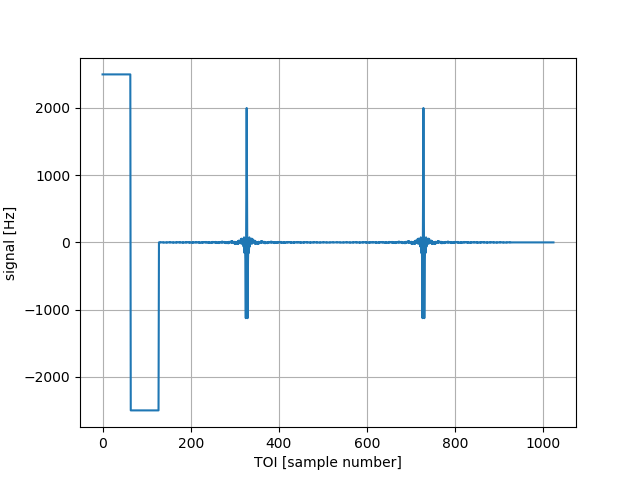
\includegraphics[width=.5\textwidth]{3.acqui/block_data.png}
	\caption{Data block simulation of KISS: signal [Hz] vs Time Ordered Information, TOI, [sample number]. There are a total of 1024 points: the first 128 dedicated to the modulation and the rest to incoming signal. We simulate the forward and backward interferograms with a typical amplitude of 2 kHz and the shape of the black body at 3 K and 30 K.}
	\label{fig:mod}
\end{figure}

\noindent The choice over the total number of points for one block, including the ones assigned to the modulation, takes into account few major constraints: the spectral resolution aimed to $\sim$1 GHz requires a displacement of the mirror of 10 cm; the cut-off of the KID time constant $\sim$100 $\mu$s, that limits the single datum acquisition rate; the fast (5 Hz) scan requirement to avoid the 1/f atmospheric noise. The result consists on a total period of 1024 points, where each point is acquired at 3.816 kHz, dedicating the first 128 to the modulation. In this way we have $\sim$400 points each interferogram, obtaining $\sim$100 points on the interested spectrum frequencies.

\noindent We can extrapolate the calibration factor $C$ [Hz/rad] through a circular fit on the modulation points $(x1,y1)$ and $(x2,y2)$, referring to fig. \ref{fig:IQ_modulation}. We obtain, in this way, the coordinates of the circle centre $(I_c,Q_c)$. We can calculate, thus, the $r_1$ and $r_2$ angles as following:

\begin{equation}
\begin{align}
r_1 &= \arctan\left( \frac{I_c-x_1}{Q_c - y_1}  \right) &\text{ ,}\\
r_2 &= \arctan\left( \frac{I_c-x_2}{Q_c - y_2}  \right) &\text{ .}
\end{align}
\end{equation}

\noindent The modulation factor $C$ is obtained as following:

\begin{equation}
\begin{align}
\Delta \phi &= r_2-r_1 &\text{ ,}\\
C&=\Delta\phi/\Delta f &\text{ ;}
\end{align}
\end{equation}

\noindent where $\Delta f$ is the modulation in hertz set by the injecting tone.

\begin{figure}[htf]
	\centering
	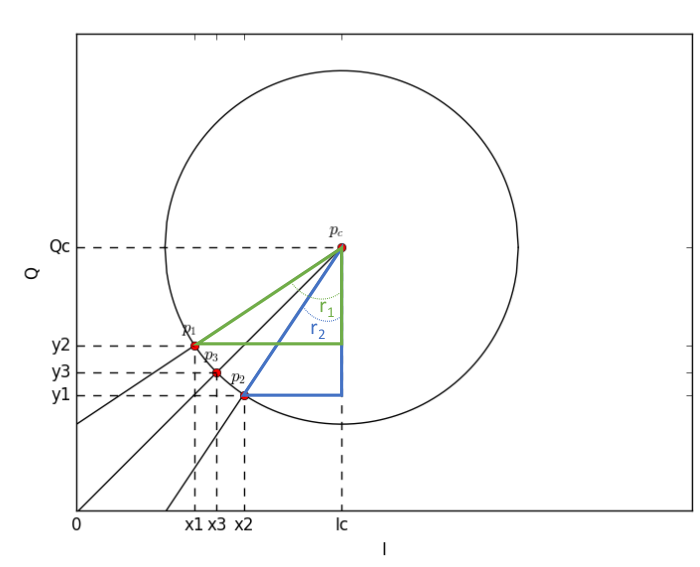
\includegraphics[width=0.5\textwidth]{3.acqui/circle.png}
	\caption{Resonance circle in the $(I,Q)$ plane. $p_1$ and $p_2$ are the modulation points, $p_3$ is the measurement point and $p_c$ is the circle centre. }
	\label{fig:IQ_modulation}
\end{figure}

\noindent Operatively, $C$ converts the observing phase, $\phi=\arctan\left( \frac{I}{Q} \right)$, to hertz data, the physical quantity (as seen in \cite{Swenson}) that can be used to obtain the incoming power in watts.


\subsection{Simulation}

In order to understand if and under which conditions this method is valuable work we use the characterising values $f_0$, resonance frequency, $Q_i$, internal quality factor, and $Q_c$, coupling quality factor, obtained in laboratory from the actual KISS arrays tests to fit the skewed Lorentzian profile \cite{Gao}:

\begin{equation}
	\left|S_{21}(f)\right|= \alpha+\beta(f-f_0)+\frac{\gamma+\delta(f-f_0)}{1+4Q_{tot}^2\cfrac{(f-f_0)^2}{f_0^2}} \text{ ,}
	\label{eq:s21_amp}
\end{equation}

\noindent where $\alpha$, $\beta$, $\gamma$ and $\delta$ are factors that do not influence the parameters on study. With eq. \ref{eq:s21_amp} we can extrapolate $Qi$ (\cite{Gao}):

\begin{equation}
Q_i =\frac{Q_{tot}}{min(\left|S_{21}(f)\right|)}
\end{equation}

\noindent In this way we simulate the KIDs used for KISS qualifying them for the modulation technique. In fig. \ref{fig:fit_amp} and \ref{fig:hist} we have the typical KISS electrical measurements in laboratory.

\begin{figure}[htf]
	\centering
	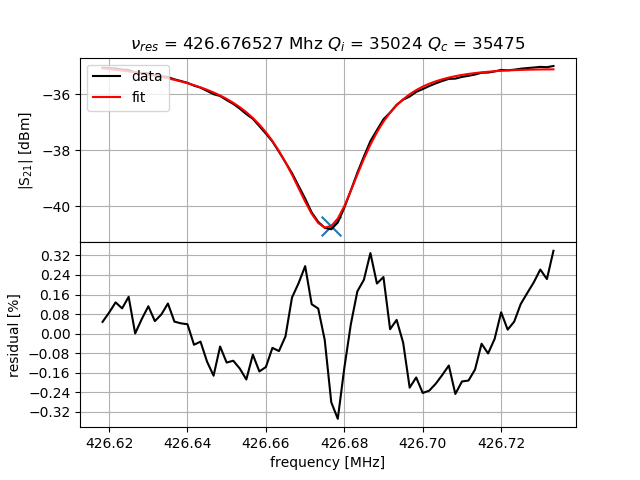
\includegraphics[width=.5\textwidth]{3.acqui/resonance_fit.png}
	\caption{Up: single pixel bias signal data (in black) fitted (in red) by \ref{eq:s21_amp}. Bottom: percentile residual between fit and data.  Typical fit using eq. \ref{eq:s21_amp} on a KISS pixel in laboratory. In this case we notice that the quality factors are coupled (aka similar), this condition maximised the responsivity (\cite{Gao}).}
	\label{fig:fit_amp}
\end{figure}

\begin{figure}[htf]
	\centering
	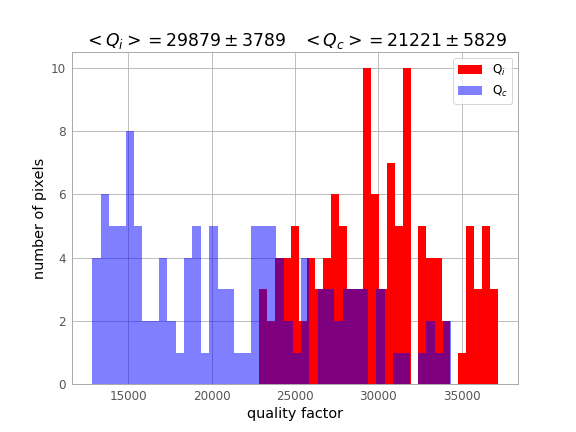
\includegraphics[width=.5\textwidth]{3.acqui/Q_hist.png}
	\caption{Quality factors histograms measured on the KISS array. In red the internal quality factor with a background of 50 K, that simulates the sky and in blue the coupling quality factor.}
	\label{fig:hist}
\end{figure}

\noindent At this point we can proceed simulating the resonator in the complex plane with the equation (\cite{Gao}):
\begin{equation}
S_{21}(f)=ae^{-2\pi j f \tau} \left[ 1-\frac{\frac{Q_{tot}}{Q_c}e^{j\phi_0}}{1+2jQ_{tot}\left(\frac{f-f_0}{f_0}\right)}\right] \text{ ,}
\label{eq:s21_IQ}
\end{equation}

\noindent using the values in tab. \ref{tab:s21_values}, where , $Q_{tot}\doteq\left( 1/Q_i + 1/Q_c \right)^{-1}$ and $\mathfrak{R}$ is the responsivity measured during laboratory test; $\tau$ is the retard introduced by the cables and $\phi_0$ is a phase, they are not taken into account for this study.

\begin{table}[htf]
	\footnotesize
	\centering
	\caption{Input values from laboratory characterisation taken from fig. \ref{fig:hist} for the resonator simulation.}
	\begin{tabular}{cc}
		\toprule
		\textbf{parameter} & \textbf{value} \\
		\toprule
		$\tau$ & 1 \\ 
		\midrule 
		$\phi_0$ & 0 \\
		\midrule
		$f_0$ & 500 MHz \\  
		\midrule 
		$Q_i$ & 30'000 @ 50 K \\ 
		\midrule 
		$Q_c$ & 21'000 \\ 
		\midrule 
		$\mathfrak{R}$  & 1.5 kHz/K \\ 
		\bottomrule
	\end{tabular}
\label{tab:s21_values}
\end{table}

\noindent We, thus, obtain the $\left|S_{21}(\nu)\right|$ shape as shown in fig. \ref{fig:s21_simu}.

\begin{figure}[htf]
	\centering
	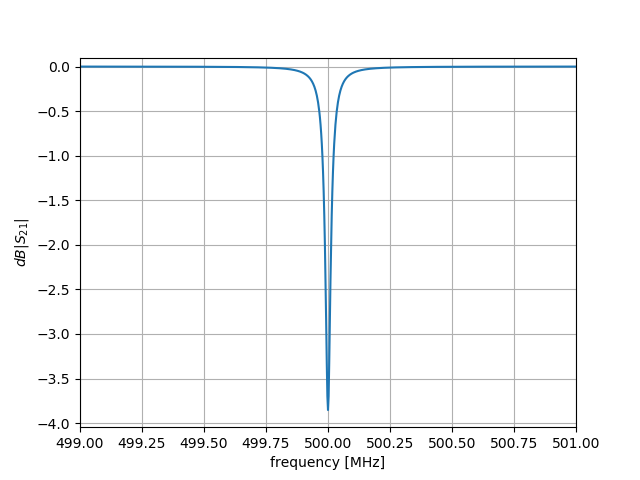
\includegraphics[width=.5\textwidth]{3.acqui/resonance.png}
	\caption{$\left|S_{21} \right|$ signal [dB] (simulated using eq. \ref{eq:s21_IQ} with input values of tab. \ref{tab:s21_values}) vs frequency [MHz]. It represents the typical KISS pixel. }
	\label{fig:s21_simu}
\end{figure}

First of all, starting from these simulated data we generate a data block with assigned modulation factor and interferogram amplitude, $A$, in hertz. The second step is to use these hertz data with eq. \ref{eq:s21_IQ} obtaining the values in quadrature $(I,Q)$. From them we compute the phase $\phi=\arctan\left(\frac{I}{Q}\right)$. Finally we come back to hertz signal through the calibration algorithm described in sec. \ref{sebsec:alg}. We, thus, compare the modulation factor and interferogram amplitude in input, $C_{in}$ and $A_{in}$ and output, $C_{out}$ and $A_{out}$, of this algorithm. This verification is necessary for understanding the reliability of the calibration method. In fig. \ref{fig:cal_bck} we report the change on the calibration factor as a function of background, at fixed modulation factor and interferogram amplitude.

\begin{figure}[htf]
	\centering
	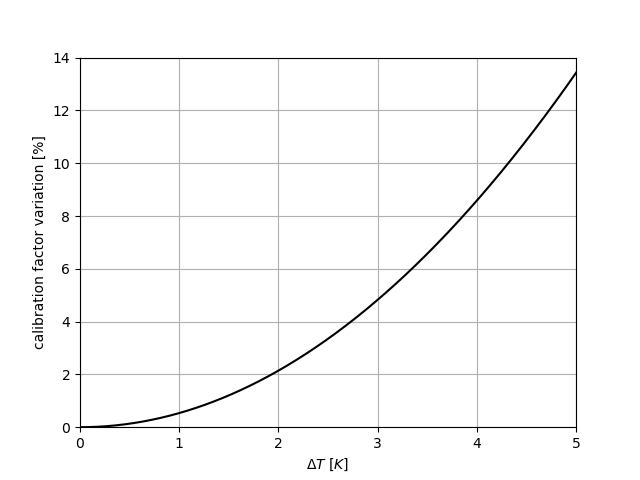
\includegraphics[width=.5\textwidth]{3.acqui/calibration_factor_variation.png}
	\caption{Calibration factor percentile variation, $\frac{C_{out}-C_{in}}{C_{in}}$, [Hz/rad] vs background variation [K]. The modulation factor, $\Delta f$, is fixed at at 2.5 kHz. The calibration factor, $C_{out}$, is independent to different $A_{in}$.}
	\label{fig:cal_bck}
\end{figure}

\noindent In fig. \ref{fig:amp_bck} we show the variation on the estimation of the interferogram amplitude, at fixed modulation factor: we see how this estimation is degradated at large background variations.

\begin{figure}[htf]
	\centering
	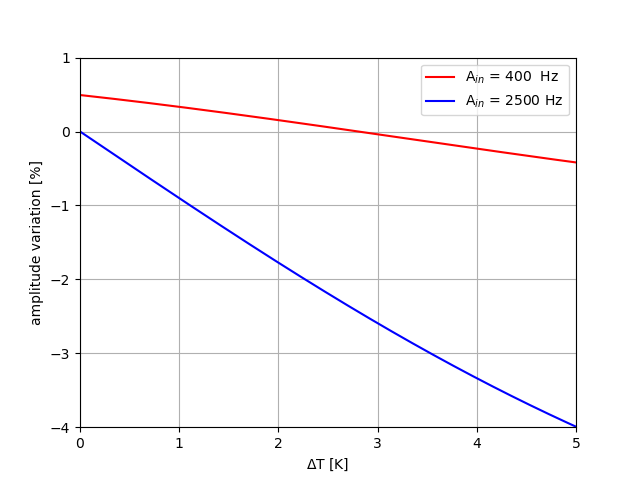
\includegraphics[width=.5\textwidth]{3.acqui/amplitude_variation.png}
	\caption{Interferogram amplitude percentile variation, $\frac{(A_{out}-A_{in})}{A_{in}}$, estimation vs background [K]. The modulation factor $\Delta f$ is fixed at 2.5 kHz. We can see how the higher value of the amplitude degrades the method}
	\label{fig:amp_bck}
\end{figure}

\noindent In fig. \ref{fig:amp_mod} we show the last result of the simulation: every curve is at different, fixed interferogram amplitude and the figure represents the variation on the amplitude estimation in function of different calibration factors. As expected, we want to be as close as possible between the calibration factor and the amplitude variation. Other choices could compromise the amplitude estimation of maximum $\sim$1\% that is, still, an acceptable compromise.

\begin{figure}[htf]
	\centering
	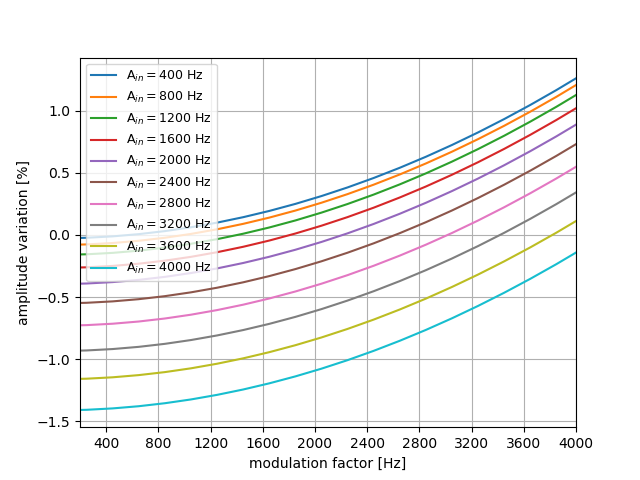
\includegraphics[width=.5\textwidth]{3.acqui/several_modulations.png}
		\caption{Every curve is at different interferogram amplitude $A_{in}$. Interferogram amplitude percentile variation, $\frac{A_{out}-A_{in}}{A_{in}}$, vs modulation factor $\Delta f$.  The background is fixed at zero. We can see how the error on the estimation converges to 0 when $\Delta f$ approaches $A_{in}$. }
	\label{fig:amp_mod}
\end{figure}

\subsection{Tuning procedure}
\label{sec:tuning}

The new modulation technique for KISS, described and simulated in the previous sections is the major improvement on the data calibration and production. On the other side, to optimise the working point of the KID it is necessary to retune: while you observe, the atmospheric fluctuations modify the resonance. What is done at the end of each observation, in the standard perspective, is a full frequency sweep to retune the resonance frequency: this represents a time-demanding procedure. By the way we can, similarly to NIKA2, adopt a strategy that permits to save $\sim$75\% of time in the pre-observation phase of retuning, this strategy is detailed explained in (\cite{2014SPIE.9153E..02C}). At first, you measure the angle $\Phi$ between the vectors $(I,Q)$ and $(dI/df_{LO},dQ/df_{LO})$ referring to eq. \ref{eq:didq} and you define, for convenience, a new angle $\theta\doteq \pi/2-\Phi$ that changes smoothly around $[-\pi,\pi]$. Secondly, the excitation tone is fixed at $\theta=0$ and you estimate the $\theta(f)$ slope $\Delta\theta/\Delta f'$. Then, you vary the tone frequency $f^i$ monitoring $\theta^i$. And finally, you can evaluate the new resonance frequency:

\begin{equation}
f^i_0 \simeq f^i - \frac{\theta^i(t)}{\Delta\theta/\Delta f'} \text{ .}
\end{equation}

The procedure described in this section is used for KISS. It represents a resilient tool that can be adopt on KIDs-based experiments: even for large background fluctuations, you can iterate the algorithm to converge.


